\documentclass[titlepage, 11pt]{article}
\usepackage[a4paper, total={6in, 9.5in}]{geometry}
\usepackage{graphicx}
\usepackage{amsmath,amsfonts,amssymb}
\usepackage{listings}
\usepackage{booktabs}
\usepackage[T1]{fontenc}
\usepackage{listings}
\usepackage{color}
\usepackage{minted}
\usepackage[colorlinks=true, linkcolor=blue, urlcolor=blue, citecolor=blue, pdfborder={0 0 255}]{hyperref}
\usepackage{colortbl}
\usepackage{url}
\usepackage{xcolor}
\usepackage{caption}
\usepackage{subcaption}
\usepackage{dirtytalk}
\usepackage{hyperref}
\usepackage[semicolon, round]{natbib}
\usepackage[ruled]{algorithm2e}
\captionsetup[table]{skip=10pt}
\renewcommand{\vec}[1]{\mathbf{#1}}
\SetKwComment{Comment}{$\triangleright$\ }{}
% \hypersetup{%
% 	colorlinks=true,
% 	linkcolor=blue,
% 	linkbordercolor={0 0 1}
% }

% \renewcommand\lstlistingname{Algorithm}
% \renewcommand\lstlistlistingname{Algorithms}
% \def\lstlistingautorefname{Alg.}

% \lstdefinestyle{Python}{
% 	language        = Python,
% 	frame           = lines, 
% 	basicstyle      = \footnotesize,
% 	keywordstyle    = \color{blue},
% 	stringstyle     = \color{green},
% 	commentstyle    = \color{red}\ttfamily
% }

% \setlength{\parindent}{0.0in}
% \setlength{\parskip}{0.05in}

\newcommand{\argmin}{\mathop{\mathrm{argmin}}}
\newcommand{\argmax}{\mathop{\mathrm{argmax}}}
\newcommand{\minimize}{\mathop{\mathrm{minimize}}}
\newcommand{\maximize}{\mathop{\mathrm{maximize}}}
\newcommand{\st}{\mathop{\mathrm{subject\,\,to}}}
\newcommand{\dist}{\mathop{\mathrm{dist}}}
\newcommand{\norm}[1]{\left\lVert#1\right\rVert}
\renewcommand{\vec}[1]{\mathbf{#1}}

\def\R{\mathbb{R}}
\def\E{\mathbb{E}}
\def\P{\mathbb{P}}
\def\S{\mathbb{S}}
\def\Cov{\mathrm{Cov}}
\def\Var{\mathrm{Var}}
\def\half{\frac{1}{2}}
\def\quat{\frac{1}{4}}
\def\sign{\mathrm{sign}}
\def\supp{\mathrm{supp}}
\def\th{\mathrm{th}}
\def\tr{\mathrm{tr}}
\def\dim{\mathrm{dim}}
\def\dom{\mathrm{dom}}

\title{
{EE1103: Numerical Methods} \\~\\
{\vlarge Programming Assignment {\#} 3}\\
}\author{ANIRUDH B S, EE21B019\\
Collaborators: & AMIZHTHNI P R K, EE21B015
 & ANKITA HARSHA MURTHY, EE21B020}
\date{\today}

\begin{document}
\maketitle

\setcounter{page}{0}
\tableofcontents
\listoffigures
\listoftables
\newpage

\section{Problem 1}
Integrate the sine wave from $[0, \pi]$ using Midpoint, Trapezoidal, and Simpson’s methods. Evaluate the integral for different $n$ (the number of subintervals) and Tabulate the absolute error for different experiments and compare the efficiency of the methods. Plot the relevant graphs to check the behaviour of the absolute error for each method as a function of $n$.
\begin{align}
    f(x) = \sin(x)
\end{align}
Find \[\int_{0}^{\pi} f(x)\,dx. \]

\subsection{Approach}

In this problem, I shall exploit the following rules to evaluate  
$\int_{0}^{\pi} \sin{x} dx$ :
\begin{itemize}
    \item [1] Mid Point Rule 
    \item [2] Trapezoidal Rule 
    \item [3] Simpson's $\frac{1}{3}$rd Rule 
\end{itemize}

We use a simple \texttt{iterative procedure} to evaluate  
$\int_{0}^{\pi} \sin{x} dx$ by dividing it into $n$ sub-intervals. 
We shall look up the cases when n = $2^k$ for $2 \leq k \leq 10$ and $k \in \mathbb{Z}$. 
%%%%%%%%%%%%%%%%%%%%%%%%%%%%%%%%%%%%%%%%%%%%%%%%%%%%%%

\subsection{Algorithm}
In this section, I present the algorithm that I shall use to compute the value of $\int_{0}^{\pi} \sin{x} dx$ using Mid-Point Rule, Trapezoidal Rule and Simpson's $\frac{1}{3}$rd rule. 

The pseudocode for the summation is provided in Algorithm~\ref{alg1}, ~\ref{alg2} and ~\ref{alg3}
\begin{center}
\begin{algorithm}[H]\label{alg1}

\SetAlgoLined

INPUT trueval \\ 
pi $\gets \pi$ \\
\For{$j=4$ to $1024$}{
dx $\gets$ $\frac{\pi}{j}$ \\
area $\gets$ 0.00 \\
i $\gets$ 0.00 \\
 \For{$k=1$ to $j$}{
   a $\gets$ i  \\
   b $\gets$ i+dx  \\
   c $\gets$ $\frac{a+b}{2}$ \\
   area $\gets$ area + dx * sin(c) \\ 
   i $\gets$ i + dx \\
 }
 $e_t$ $\gets$ |area - trueval| \\
 PRINT area, $e_t$ \\
 j $\gets$ j*2\\
}

 \caption{Approximating  $\int_{0}^{\pi} \sin{x} dx$ using Mid-Point Rule}
\end{algorithm}    
\end{center}

\begin{center}
\begin{algorithm}[H]\label{alg2}

\SetAlgoLined

INPUT trueval \\ 
pi $\gets \pi$ \\
\For{$j=4$ to $1024$}{
dx $\gets$ $\frac{\pi}{j}$ \\
area $\gets$ 0.00 \\
i $\gets$ 0.00 \\
 \For{$k=1$ to $j$}{
   a $\gets$ i  \\
   b $\gets$ i+dx  \\
   c $\gets$ $\frac{sin(a)+sin(b)}{2}$ \\
   area $\gets$ area + dx * c \\ 
   i $\gets$ i + dx \\
 }
 $e_t$ $\gets$ |area - trueval| \\
 PRINT area, $e_t$ \\
 j $\gets$ j*2\\
}

 \caption{Approximating  $\int_{0}^{\pi} \sin{x} dx$ using Trapezoid Rule}
\end{algorithm}    
\end{center}

\begin{center}
\begin{algorithm}[H]\label{alg3}

\SetAlgoLined

INPUT trueval \\ 
pi $\gets \pi$ \\
\For{$j=4$ to $1024$}{
dx $\gets$ $\frac{\pi}{j}$ \\
area $\gets$ 0.00 \\
i $\gets$ 0.00 \\
 \For{$k=0$ to $j$}{
   a $\gets$ i  \\
   \If{k==0||k==j}{
      area += sin(a) \\
   }
   \If{k\%2==0}{
      area += 2*sin(a) \\
   }
     \If{k\%2!=0}{
      area += 4*sin(a) \\
   }
   
   i $\gets$ i + dx \\
 }
 area $\gets$ area * $\frac{dx}{3}$ \\
 $e_t$ $\gets$ |area - trueval| \\
 PRINT area, $e_t$ \\
 j $\gets$ j*2\\
}

 \caption{Approximating  $\int_{0}^{\pi} \sin{x} dx$ using Simpson's $\frac{1}{3}$rd Rule}
\end{algorithm}    
\end{center}

%%%%%%%%%%%%%%%%%%%%%%%%%%%%%%%%%%%%%%%%%%%%%%%%%%%%%%
\subsection{Results}

We obtain the following results after subdividing [0.$\pi$] into 1024 sub-intervals. 
\begin{itemize}
    \item [1] Mid Point Method - 2.000001
    \item [2] Trapezoid Method - 1.999998
    \item [3] Simpson's Rule - 2.000000
\end{itemize}

Efficiency of the methods follow : Simpson's Method > Mid - Point Method $\approx$ Trapezoid Method.

Here, I shall plot the graphs showing the absolute error percentage as a function of the number of sub-intervals considered while approximating $\int_{0}^{\pi} \sin{x} dx$ In Figure~\ref{fig:q1a}, ~\ref{fig:q1b} and ~\ref{fig:q1c}. The results are also summarized in Tables ~\ref{tab:tab1a}, ~\ref{tab:tab1b} and ~\ref{tab:tab1c}.


\begin{figure}[!tbh]
  	\centering
  	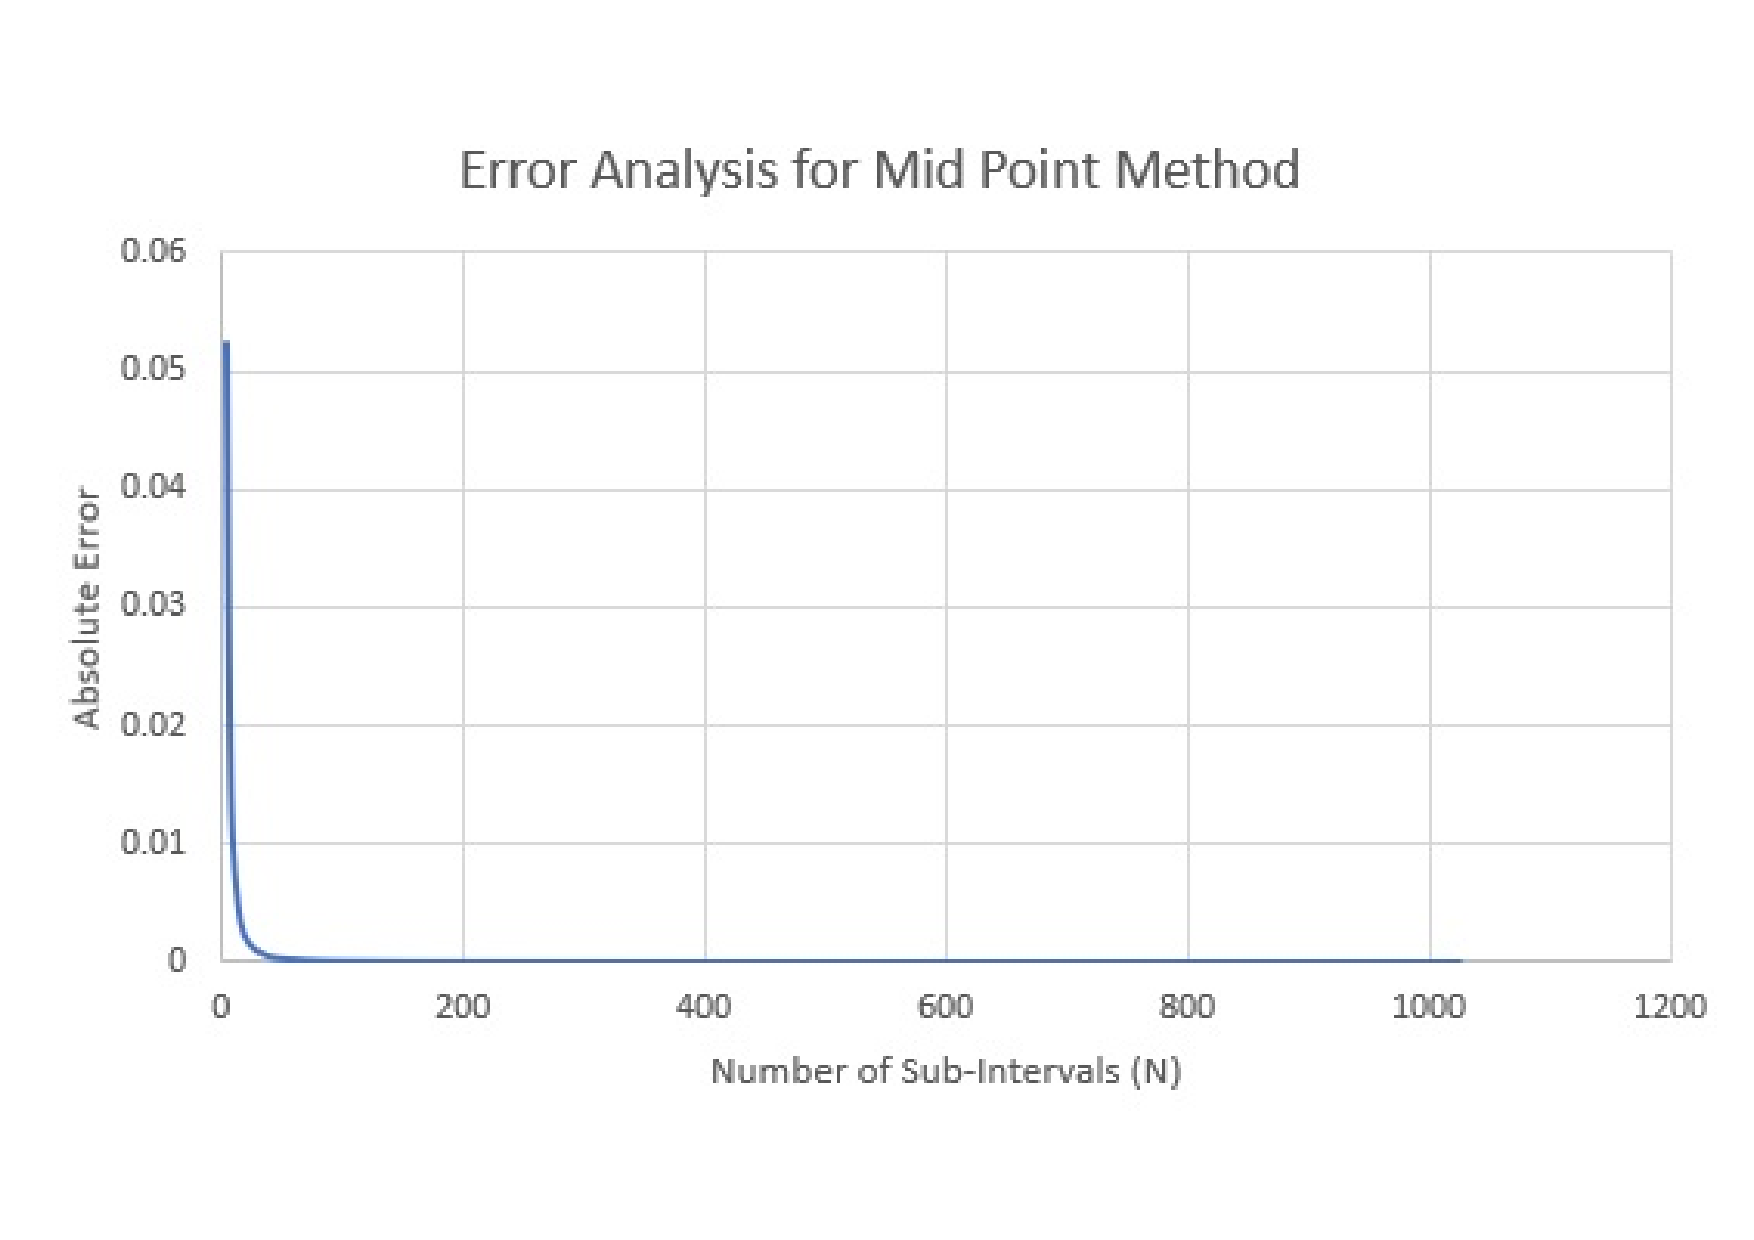
\includegraphics[width=0.9\textwidth]{MP1.pdf} 
  	\caption{Absolute Error vs Number of Sub-Intervals using Mid-Point Rule.}
  	\label{fig:q1a} 
\end{figure}
\begin{figure}[!tbh]
  	\centering
  	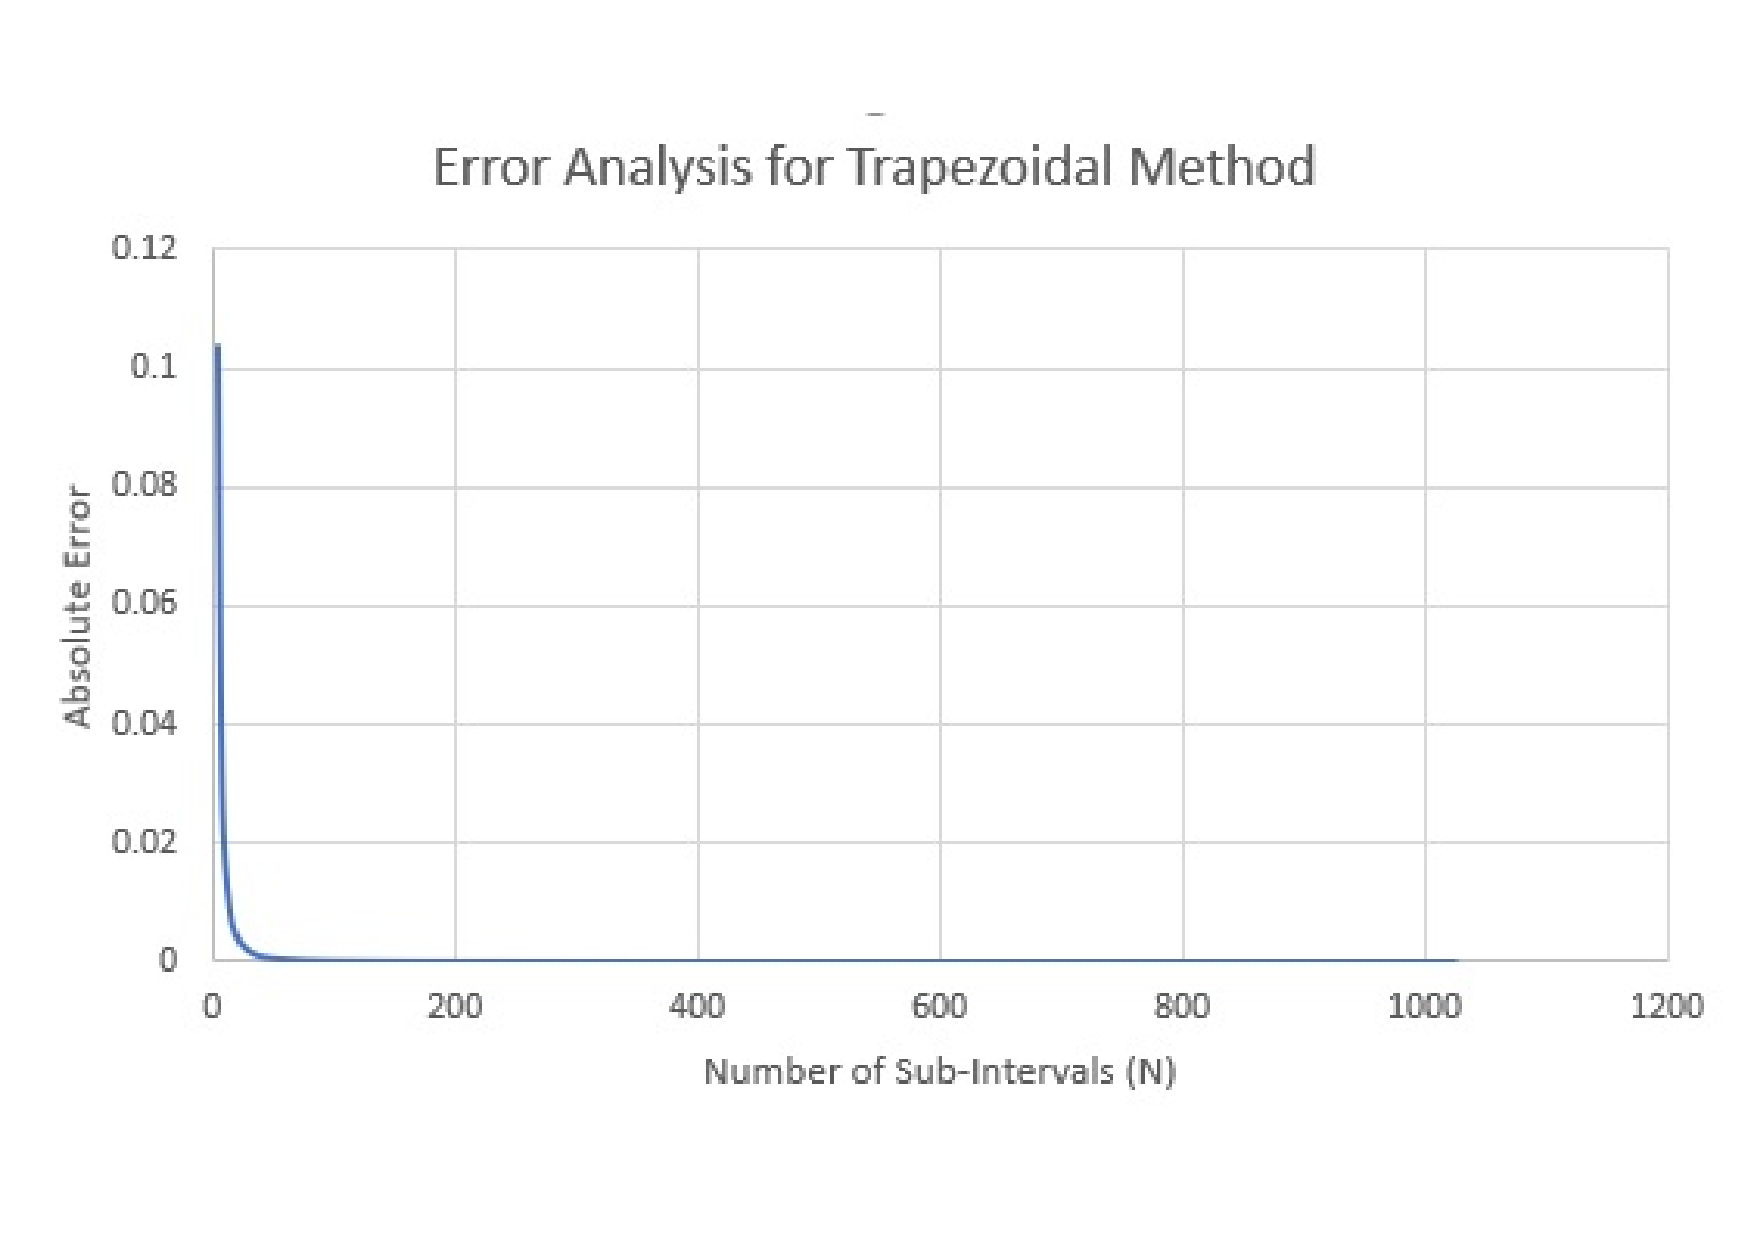
\includegraphics[width=0.9\textwidth]{TP1.pdf} 
  	\caption{Absolute Error vs Number of Sub-Intervals using Trapezoidal Rule.}
  	\label{fig:q1b} 
\end{figure}
\begin{figure}[!tbh]
  	\centering
  	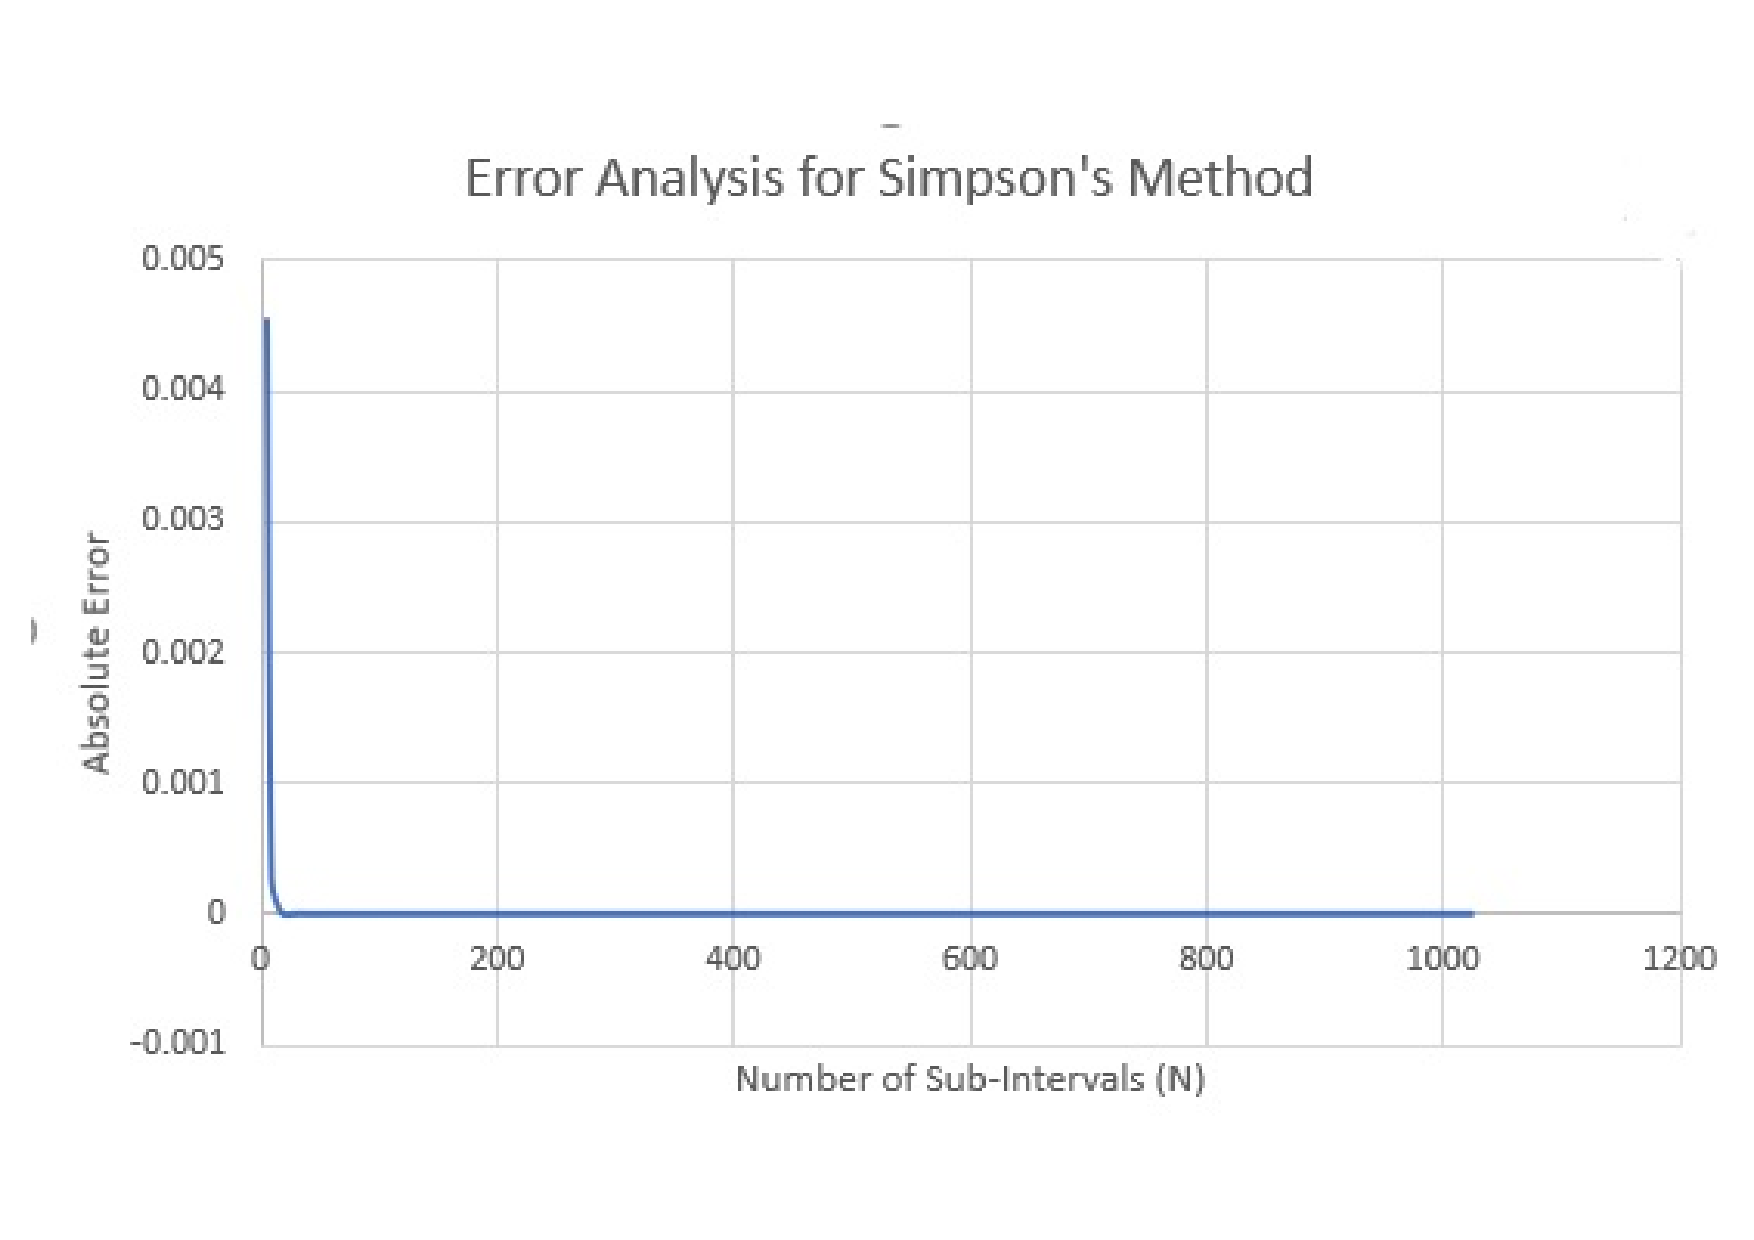
\includegraphics[width=0.9\textwidth]{SR1.pdf} 
  	\caption{Absolute Error vs Number of Sub-Intervals using Simpson's $\frac{1}{3}$rd Rule.}
  	\label{fig:q1c} 
\end{figure}

\begin{table}[!htb]
    \caption{Number of sub-intervals vs Approximate Value vs Absolute Error using Mid-Point Rule}
    \centering
    \begin{tabular}{ccc}
    \toprule
    \textbf{$n$}& \textbf{Approximate value}& \textbf{Absolute Error}   \\
    \midrule
         4	& 2.052344	& 0.052344 \\
         8	& 2.012909	&  0.012909 \\
         16	& 2.003216	& 0.003216 \\
         32	& 2.000803	& 0.000803 \\
         64	 & 2.000201	& 0.000201 \\
         128 &	 2.000050 & 0.00005 \\
         256 &  2.000013 &	 0.000013 \\
         512 & 2.000003 &	 0.000003 \\
         1024	& 2.000001 &	 0.000001 \\ 
    \bottomrule
    \end{tabular}
    \label{tab:tab1a}
\end{table}
\begin{table}[!htb]
    \caption{Number of sub-intervals vs Approximate Value vs Absolute Error using Trapezoidal Rule}
    \centering
    \begin{tabular}{ccc}
    \toprule
    \textbf{$n$}& \textbf{Approximate value}& \textbf{Absolute Error}   \\
    \midrule
        4 &  1.896119 & 0.103881 \\
        8 & 1.974232 & 0.025768\\
16	& 1.993570	 & 0.006430 \\
32	& 1.998393	 & 0.001607 \\
64	& 1.999598	 & 0.000402 \\
128	& 1.999900	 & 0.0001 \\
256	& 1.999975	 & 0.000025 \\ 
512	& 1.999994	& 0.000006 \\
1024 &	 1.999998	& 0.000002 \\
    \bottomrule
    \end{tabular}
    \label{tab:tab1b}
\end{table}
\begin{table}[!htb]
    \caption{Number of sub-intervals vs Approximate Value vs Absolute Error using Simpson's $\frac{1}{3}$ Rule}
    \centering
    \begin{tabular}{ccc}
    \toprule
    \textbf{$n$}& \textbf{Approximate value}& \textbf{Absolute Error}   \\
    \midrule
       4 &	 2.004560 & 0.00455975\\
8	& 2.000269	& 0.00026917 \\
16	& 2.000017	& 1.6591 x 10^{\mbox{-5}} \\
32	& 2.000001	& 1.0334 x 10^{\mbox{-6}} \\
64	& 2.000000	& 6.453 x 10^{\mbox{-8}} \\
128	& 2.000000	& 4.032 x 10^{\mbox{-9}} \\
256	& 2.000000	& 2.52 x 10^{\mbox{-10}} \\
512	& 2.000000	& 1.6 x 10^{\mbox{-11}} \\
1024 & 2.000000	& 1 x 10^{\mbox{-12}} \\

    \bottomrule
    \end{tabular}
    \label{tab:tab1c}
\end{table}

%%%%%%%%%%%%%%%%%%%%%%%%%%%%%%%%%%%%%%%%%%%%%%%%%%%%%%

\subsection{Inferences}
I deduce the following inferences from this problem :
\begin{itemize}
    \item There is a sharp decline in the absolute error as we increase the number of sub-intervals. In principle, as n would tend towards $\intfy$, the approximate value of the integral shall converge to the true value of the integral. This is true for all the three methods demonstrated.  
    \item It appears that the \textbf{Mid Point Method} and the  \textbf{Trapezoid Method} give almost the same error. This is because both these methods approximate area using four-sided polygons - rectangle and trapezium respectively. However, \textbf{The Simpson's $\frac{1}{3}$ Rule} does much better in giving a faster convergence to the true value compared to the former methods. This is because, the Simpson's Method uses parabolas to estimate the area, which is called as \textit{The Quadratic Approximation}, and thus, does better. 
    \item Now, I shall list the various upper bounds for the error.
    \begin{itemize}
        \item [1] Error in Mid Point Method $\leq$ $\frac{M(b-a)^3}{24n^2}$
        \item [2] Error in Trapezoid Method $\leq$ $\frac{M(b-a)^3}{12n^2}$
        \item [3] Error in Simpson's Method $\leq$ $\frac{M(b-a)^5}{180n^4}$
    \end{itemize}
    where, n denotes the number of sub-intervals taken, b-a denotes the length of each sub-interval and M is the maximum modulus value of the second derivative of the function f(x).
    \item It can also be clearly inferred that the mid-point method provides a better estimate of area compared to the Trapezoid Method. The Trapezoid Method overestimates the area when the function is concave up and underestimates when the function is concave down. On the other hand, the Mid-Point method averages out the two segments. 
     \item The Simpson's Method seems to give a better and quicker approximation of the integral compared to the Mid-Point Method which in turn gives results relatively better than the Trapezoid Method.
    \item For a given n, larger the length of the interval, the upper bound on the error for the mid-point and trapezoid rule decrease while that of Simpson's Method increases. This indirectly tells us that Simpson's method is more accurate for smaller intervals as compared to larger intervals. 
    \item Similarly, for a given length of the interval, as we increase n, the upper error bound on the Mid-Point and Trapezoid rule decrease as $\frac{1}{n^2}$ while that of Simpson's rule decreases as $\frac{1}{n^4}$. This suggests that for larger number of sub-intetvals, the Simpson's rule is more accurate and quicker as compared to the other two methods.
    \item It can clearly be shown that 
    \begin{equation}
        T_n = \frac{L_n+R_n}{2}
    \end{equation}
    where $T_n$ denotes the area found using Trapezoid Rule, $L_n$ denotes the approximate integral by taking the left hand end points of each sub-interval alone and $R_n$ denotes the approximate integral by taking the right hand end points of each sub-interval alone.
    \item Simpson's Rule may be obtained from the Mid-Point and Trapezoid Rules by using a weighed average. It can be shown that :
    \begin{equation}
        S_{2n} = \frac{2M_n+T_n}{3}
    \end{equation}
    \item In summary, the Simpson's method provides a better and quicker approximate of area compared to the Mid-Point Method which in turn performs comparatively better than the Trapezoid Method. 
\end{itemize}

%%%%%%%%%%%%%%%%%%%%%%%%%%%%%%%%%%%%%%%%%%%%%%%%%%%%%%

\subsection{Code}
The code used for the problem are mentioned in Listings : \begin{itemize}
    \item [1] Mid Point Rule - ~\ref{listing:1}
    \item [2] Trapezoidal Rule - ~\ref{listing:2}
    \item [3] Simpson's $\frac{1}{3}$rd Rule - ~\ref{listing:3}
\end{itemize}

\inputminted[breaklines,
 mathescape,
 linenos,
 numbersep=5pt,
 frame=single,
 numbersep=5pt,
 xleftmargin=0pt]{c}{P1MP.c}
 \captionof{listing}{Mid-Point Rule CODE}
\label{listing:1}
\inputminted[breaklines,
 mathescape,
 linenos,
 numbersep=5pt,
 frame=single,
 numbersep=5pt,
 xleftmargin=0pt]{c}{P1TP.c}
 \captionof{listing}{Trapezoidal Rule CODE}
\label{listing:2}
\inputminted[breaklines,
 mathescape,
 linenos,
 numbersep=5pt,
 frame=single,
 numbersep=5pt,
 xleftmargin=0pt]{c}{P1SR.c}
 \captionof{listing}{Simpson's $\frac{1}{3}$rd rule CODE}
\label{listing:3}

%%%%%%%%%%%%%%%%%%%%%%%%%%%%%%%%%%%%%%%%%%%%%%%%%%%%%%

\subsection{Contributions}
In the above problem, \textit{my original contributions} are - 
\begin{itemize}
    \item Designing of the Algorithm and Code
    \item Plotting of the graph on Google Sheets. 
    \item Analysis of True Error
    \item Tabulation of Results and Errors
    \item Drawing conclusions by looking at the Result obtained and Error Analysis.
    \item Writing the report in LaTeX. 
\end{itemize}


%%%%%%%%%%%%%%%%%%%%%%%%%%%%%%%%%%%%%%%%%%%%%%%%%%%%%%

\subsection{Alternate Methods }
The Mid-Point Method, Trapezoid Method and Simpson's Rule all seem to converge to the true value of the intgral as the number of sub-intervals increase. However, each of these methods has its own pitfalls. The Trapezoid method overestimates or underestimates area when subjected to concave up and concave down curvatures respectively. However, in case of linear functions, the Trapezoid and Mid-Point Methods give exact answers while Simpson's method fails to give a quicker convergence. \\
In case of unequal sub-interval lengths, the methods could perform better or worse depending on the integrand. \\
Depending on the function to be taken as the integrand. a suitable method of integration can be chosen. I shall mention few other methods here. \\
\begin{itemize}
    \item [1] \href{https://en.wikipedia.org/wiki/Romberg%27s_method}{The Romberg Method} is a more efficient method when compared to \textbf{The Simpson's $\frac{1}{3}$rd rule.}
    \item [2] \href{https://en.wikipedia.org/wiki/Boole%27s_rule}{The Boole's Rule} is also a numerical method of integration. It provides a higher efficiency compared to the three methods which we discussed in certain situations. 
    \item [3] \href{https://en.wikipedia.org/wiki/Gaussian_quadrature}{The Gaussian Quadrature} is considered in many cases as the exact integral and evaluates an integral to unexpected degree of accuracy. 
\end{itemize}


%%%%%%%%%%%%% END OF QUESTION 1 %%%%%%%%%%%%%%%%%%%%
\newpage
% Uncomment the lines below to add references using bibtex.
% \bibliographystyle{plainnat}
% \bibliography{references}
\section{Problem 2}
Integrate the standard Gaussian pdf to estimate {Erf(1)} and {Erf(2)} using Midpoint, Trapezoidal, and Simpson’s rules.\\
Note: Assume the Gaussian PDF has 0 value outside the range [-4,4].
\begin{itemize}
  \item [a)]Tabulate the absolute error for different experiments and compare the efficiency of the methods.
  \item [b)]Plot the absolute error vs $n$ and explain if there is any anomalous behaviour. Is neglecting the region outside [-4,4] a good choice for calculating the integral with 0.1\% accuracy?
  \item [c)]Compare the values of {Erf(1)} and {Erf(2)} obtained by integration to those obtained using the empirical distribution in the previous assignment.
\end{itemize}   

\begin{align}
    {\rm Erf}(x) = \frac{1}{\sqrt{2\pi}}\int_{-\infty}^{x}e^{\frac{-t^2}{2}}\,dt
\end{align} 

\subsection{Approach}

In this problem, I shall exploit the following rules to evaluate  
$\frac{1}{\sqrt{2\pi}} \int_{-\infty}^{x} e^{\frac{-t^2}{2}} dt$ :
\begin{itemize}
    \item [1] Mid Point Rule 
    \item [2] Trapezoidal Rule 
    \item [3] Simpson's $\frac{1}{3}$rd Rule 
\end{itemize}

We use a simple \textit{iterative procedure} to evaluate  
$\frac{1}{\sqrt{2\pi}} \int_{-\infty}^{x} e^{\frac{-t^2}{2}} dt$ by dividing it into $n$ sub-intervals. 
We shall look up the cases when n = $2^k$ for $2 \leq k \leq 10$ and $k \in \mathbb{Z}$. 
%%%%%%%%%%%%%%%%%%%%%%%%%%%%%%%%%%%%%%%%%%%%%%%%%%%%%%

\subsection{Algorithm}
In this section, I present the algorithm that I shall use to compute the value of $\frac{1}{\sqrt{2\pi}} \int_{-\infty}^{x} e^{\frac{-t^2}{2}} dt$ using Mid-Point Rule, Trapezoidal Rule and Simpson's $\frac{1}{3}$rd rule. 

The pseudocode for the summation is provided in Algorithm~\ref{alg4}, ~\ref{alg5} and ~\ref{alg6}
\begin{center}
\begin{algorithm}[H]\label{alg4}

\SetAlgoLined

INPUT trueval,x \\
\For{$j=4$ to $1024$}{
dx $\gets$ $\frac{x+4}{j}$ \\
area $\gets$ 0.00 \\
i $\gets$ -4.00 \\
 \For{$k=1$ to $j$}{
   a $\gets$ i  \\
   b $\gets$ i+dx  \\
   c $\gets$ $\frac{a+b}{2}$ \\
   area $\gets$ area + dx *$ e^{\frac{-c^2}{2}}$ \\ 
   i $\gets$ i + dx \\
 }
 area $\gets$ $\frac{area}{\sqrt{2\pi}}$ \\
 $e_t$ $\gets$ |area - trueval| \\
 PRINT area, $e_t$ \\
 j $\gets$ j*2\\
}

 \caption{Approximating  $\frac{1}{\sqrt{2\pi}} \int_{-\infty}^{x} e^{\frac{-t^2}{2}} dt$ using Mid-Point Rule}
\end{algorithm}    
\end{center}

\begin{center}
\begin{algorithm}[H]\label{alg5}

\SetAlgoLined

INPUT trueval,x  \\ 
\For{$j=4$ to $1024$}{
dx $\gets$ $\frac{x+4}{j}$ \\
area $\gets$ 0.00 \\
i $\gets$ -4.00 \\
 \For{$k=1$ to $j$}{
   a $\gets$ i  \\
   b $\gets$ i+dx  \\
   c $\gets$ $\frac{ e^{\frac{-a^2}{2}}+e^{\frac{-b^2}{2}}}{2}$ \\
   area $\gets$ area + dx * c \\ 
   i $\gets$ i + dx \\
 }
  area $\gets$ $\frac{area}{\sqrt{2\pi}}$ \\
 $e_t$ $\gets$ |area - trueval| \\
 PRINT area, $e_t$ \\
 j $\gets$ j*2\\
}

 \caption{Approximating  $\frac{1}{\sqrt{2\pi}} \int_{-\infty}^{x} e^{\frac{-t^2}{2}} dt$ using Trapezoid Rule}
\end{algorithm}    
\end{center}

\begin{center}
\begin{algorithm}[H]\label{alg6}

\SetAlgoLined

INPUT trueval, x \\ 
\For{$j=4$ to $1024$}{
dx $\gets$ $\frac{x+4}{j}$ \\
area $\gets$ 0.00 \\
i $\gets$ -4.00 \\
 \For{$k=0$ to $j$}{
   a $\gets$ i  \\
   \If{k==0||k==j}{
      area += $ e^{\frac{-a^2}{2}}$ \\
   }
   \If{k\%2==0}{
      area += 2*$ e^{\frac{-a^2}{2}}$ \\
   }
     \If{k\%2!=0}{
      area += 4*$ e^{\frac{-a^2}{2}}$ \\
   }
   
   i $\gets$ i + dx \\
 }
 area $\gets$ area * $\frac{dx}{3}$ \\
 area $\gets$ $\frac{area}{\sqrt{2\pi}}$ \\
 $e_t$ $\gets$ |area - trueval| \\
 PRINT area, $e_t$ \\
 j $\gets$ j*2\\
}

 \caption{Approximating  $\frac{1}{\sqrt{2\pi}} \int_{-\infty}^{x} e^{\frac{-t^2}{2}} dt$ using Simpson's $\frac{1}{3}$rd Rule}
\end{algorithm}    
\end{center}


%%%%%%%%%%%%%%%%%%%%%%%%%%%%%%%%%%%%%%%%%%%%%%%%%%%%%%
\subsection{Results}
\begin{itemize}
    \item [(a)] Efficiency of the methods follow : Simpson's Method > Mid - Point Method $\approx$ Trapezoid Method.
    \item [(b)] Yes, neglecting the region outside [-4,4] is fine in evaluating the integral in this case as the value of the function $f(x)= e^{\frac{-x^2}{2}}$ is very negligible for x>4 when compared to those around 0.
    \item [(c)] In the previous assignment, we obtained the values of ERF(1) as 0.8373 and ERF(2) as 0.9744. In the present assignment, we obtain the value of ERF(1) as 0.841313 and ERF(2) 0.977218 using all the three iterative procedures. The values obtained by numerical integration are more closer to the real values as compared to those obtained in the previous assignment. 
\end{itemize} 

Here, I shall plot the graphs showing the absolute error percentage as a function of the number of sub-intervals considered while approximating $\frac{1}{\sqrt{2\pi}} \int_{-\infty}^{x} e^{\frac{-t^2}{2}} dt$ . In Figure~\ref{fig:q2a}, ~\ref{fig:q2b} and ~\ref{fig:q2c}. The results are also summarized in Tables ~\ref{tab:Q21} and ~\ref{tab:Q22}.


\begin{figure}[ht]
\begin{subfigure}{.5\textwidth}
  \centering
  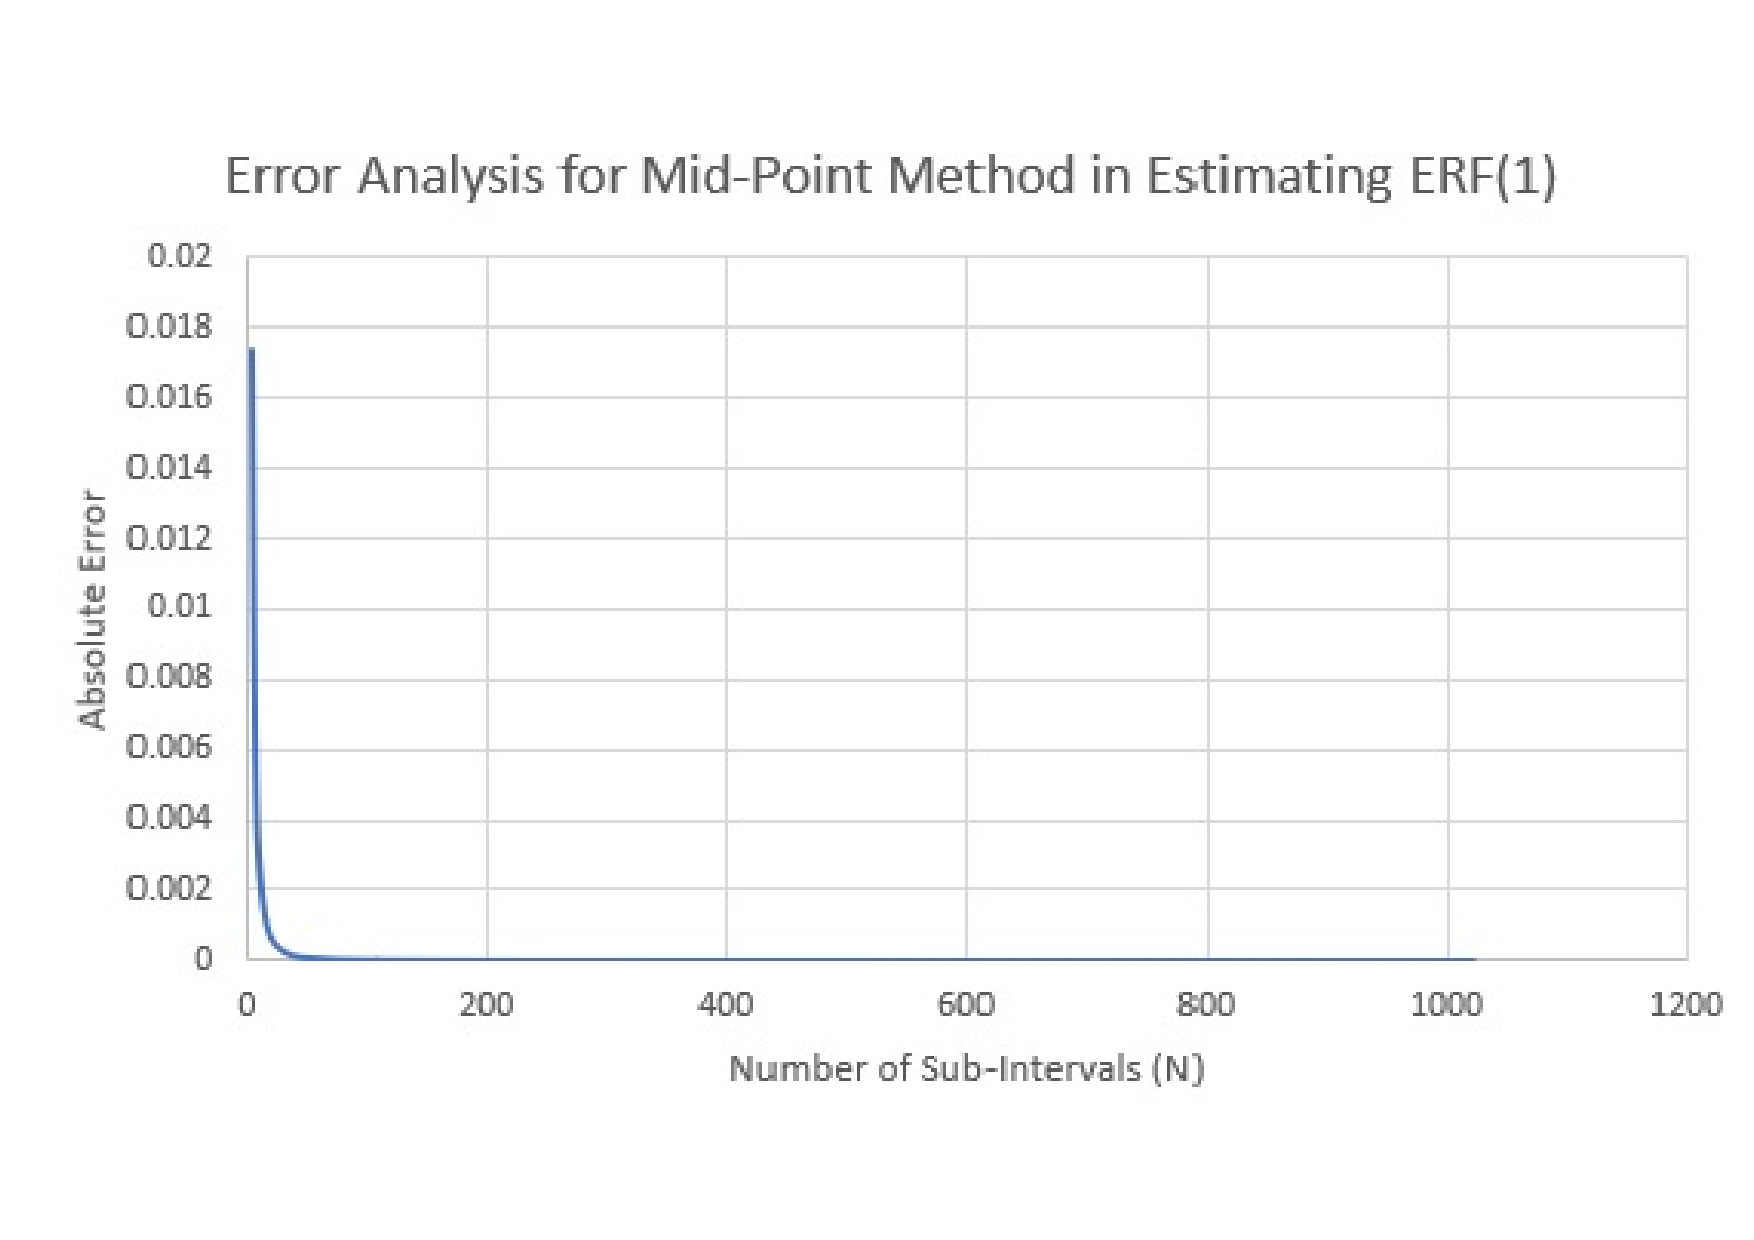
\includegraphics[width=\linewidth]{MP2ERF1.pdf}
  \caption{Error Analysis for ERF 1}
  \label{fig:q2a1}
\end{subfigure}
\begin{subfigure}{.5\textwidth}
  \centering
  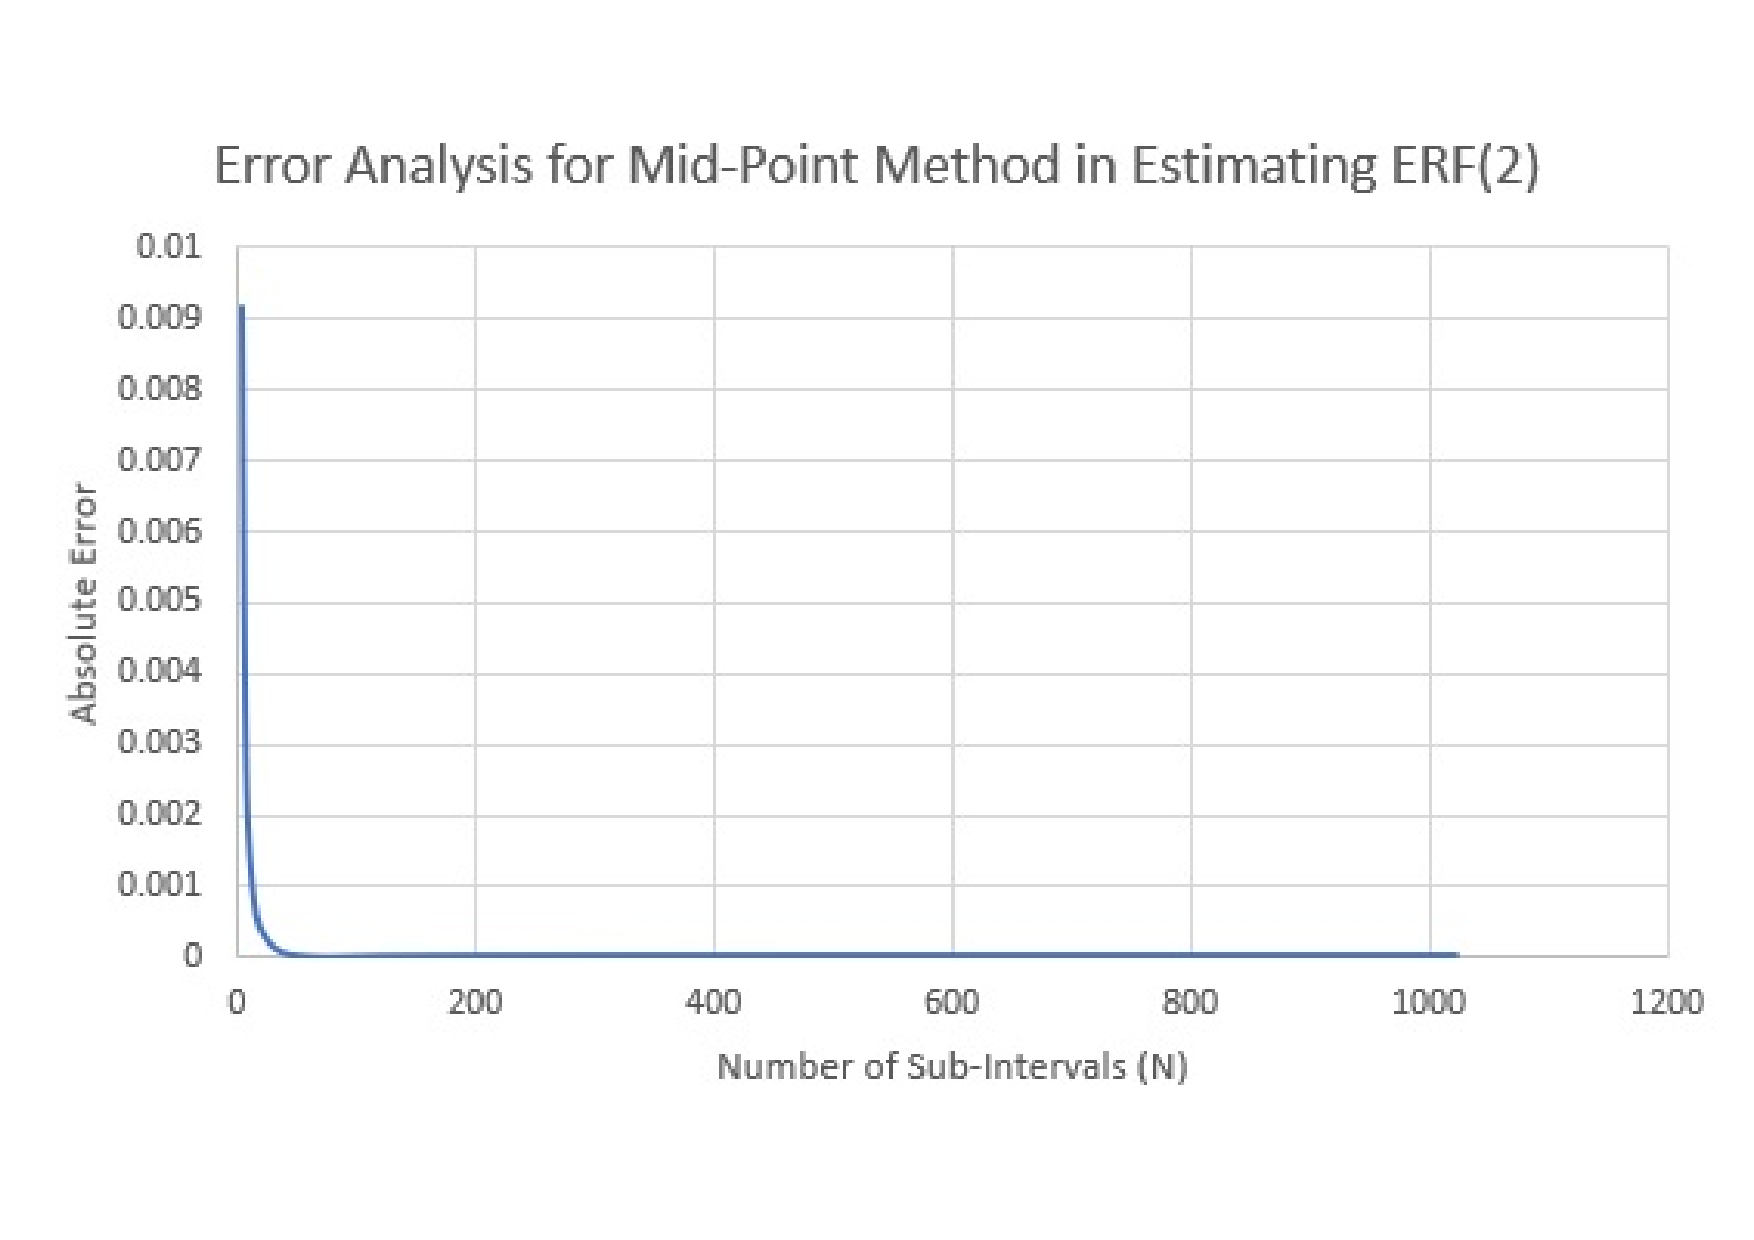
\includegraphics[width=\linewidth]{MP2ERF2.pdf}
  \caption{Error Analysis for ERF 2}
  \label{fig:q2a2}
\end{subfigure}
\caption{Absolute Error vs Number of Sub-Intervals using Mid-Point Rule.}
\label{fig:q2a}
\end{figure}
\begin{figure}[ht]
\begin{subfigure}{.5\textwidth}
  \centering
  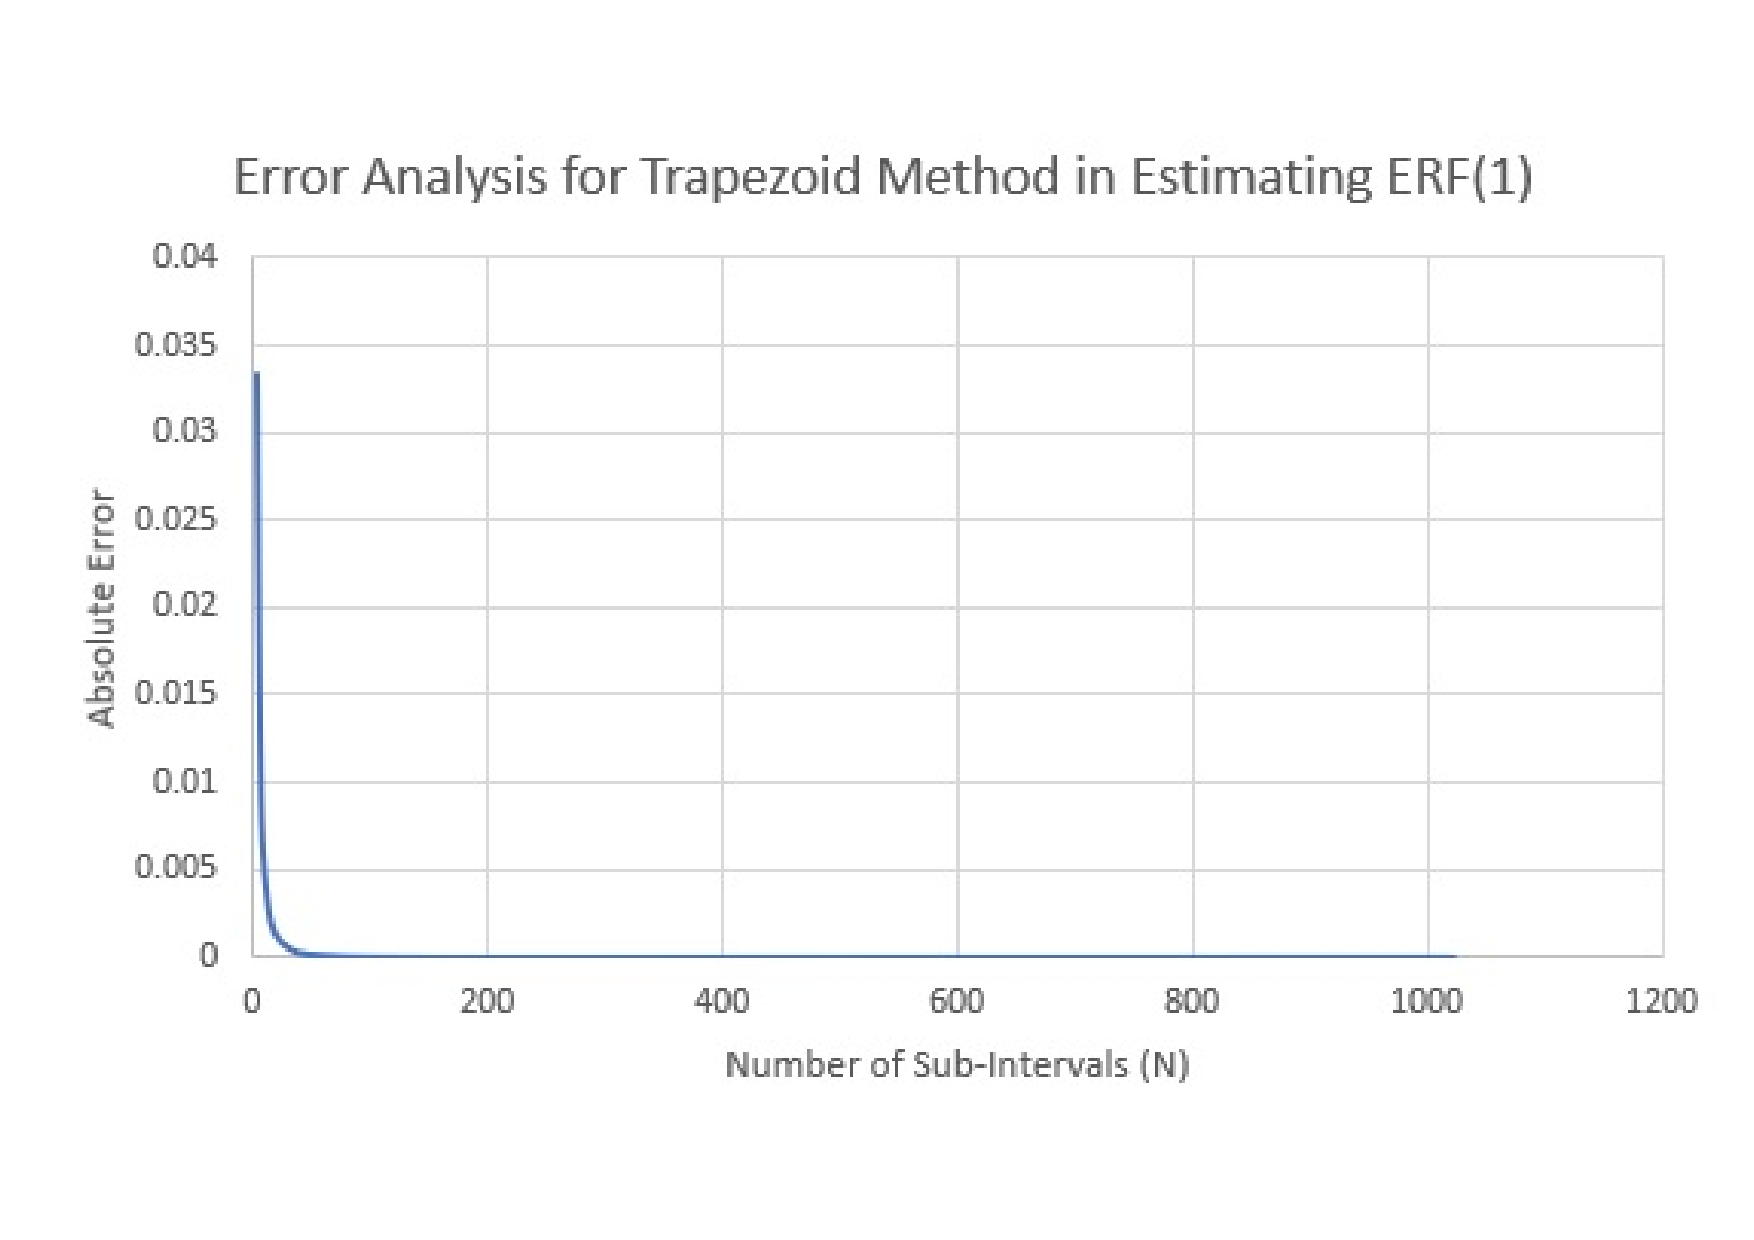
\includegraphics[width=\linewidth]{TP2ERF1.pdf}
  \caption{Error Analysis for ERF 1}
  \label{fig:q2b1}
\end{subfigure}
\begin{subfigure}{.5\textwidth}
  \centering
  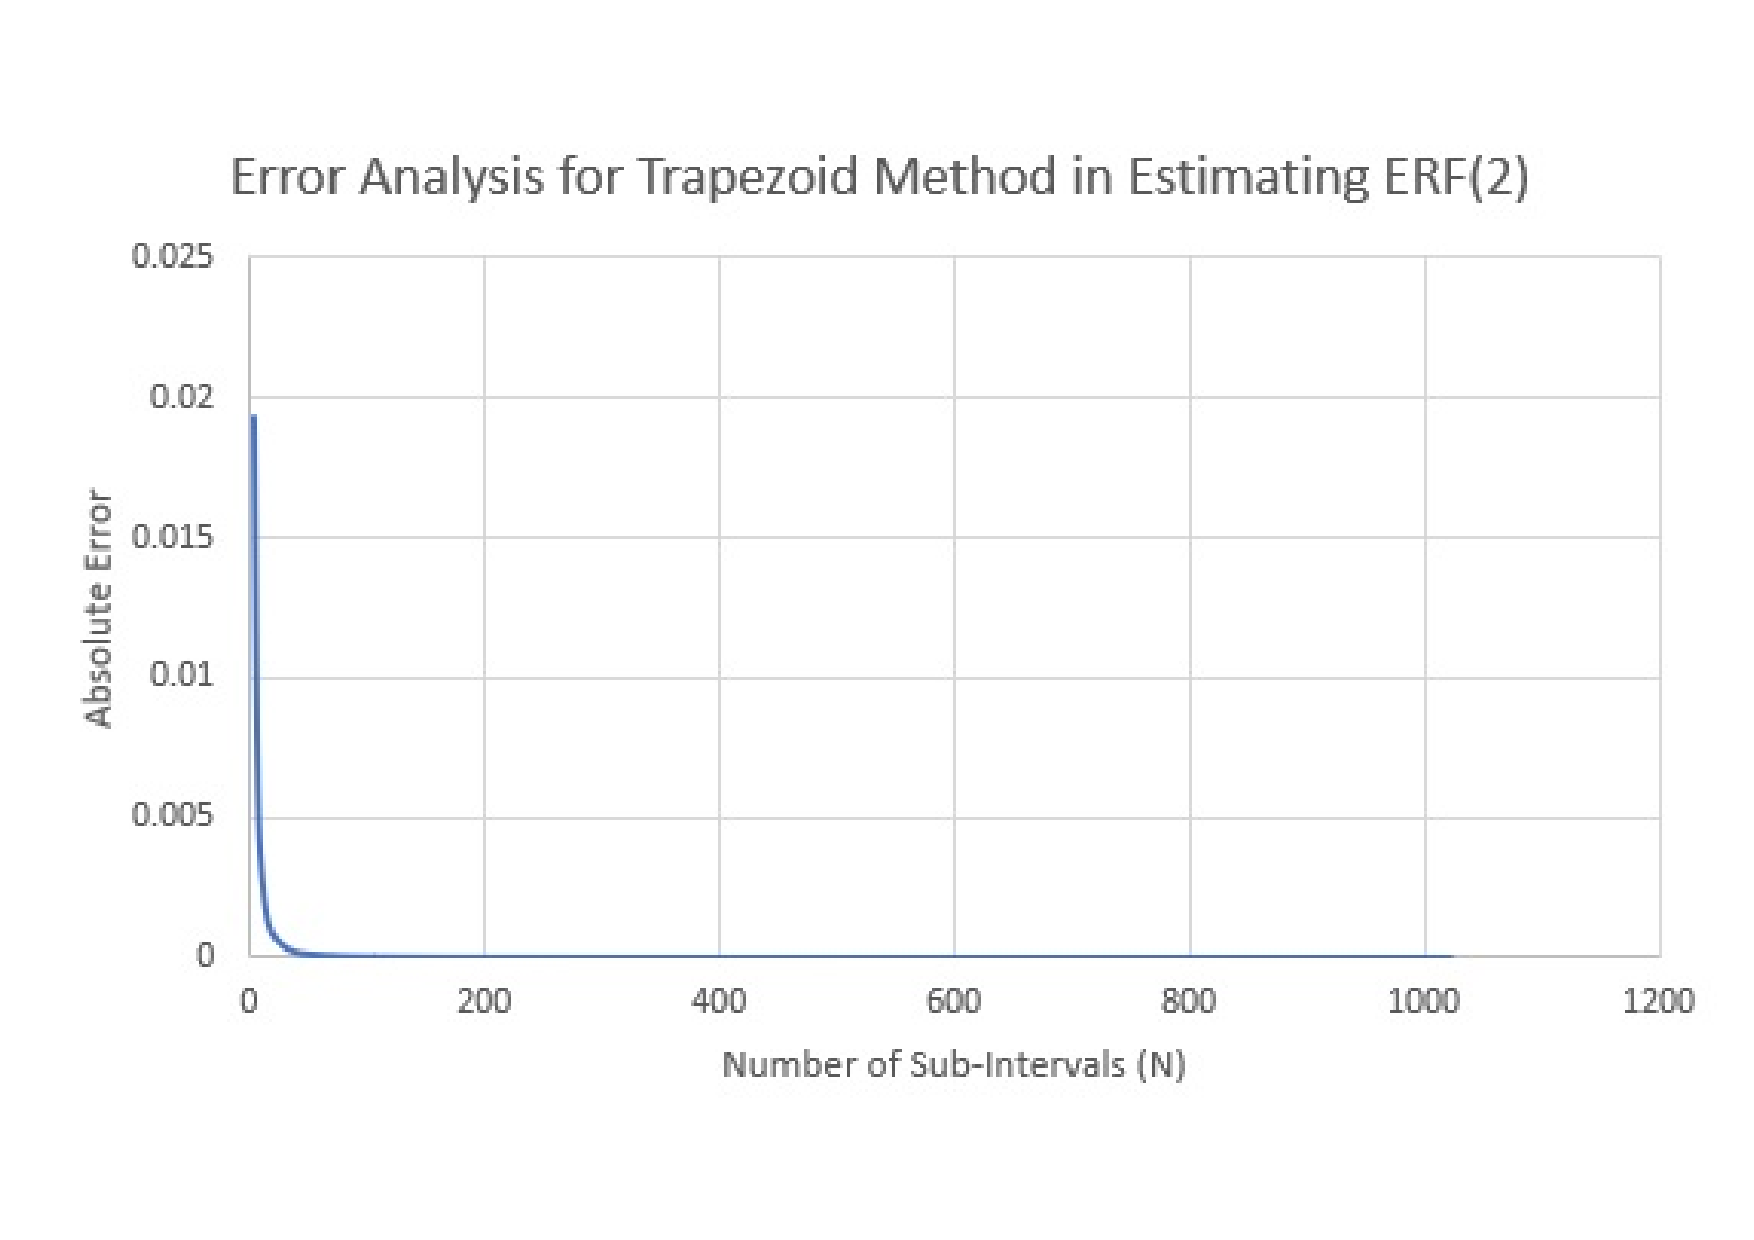
\includegraphics[width=\linewidth]{TP2ERF2.pdf}
  \caption{Error Analysis for ERF 2}
  \label{fig:q2b2}
\end{subfigure}
\caption{Absolute Error vs Number of Sub-Intervals using Trapezoidal Rule.}
\label{fig:q2b}
\end{figure}
\begin{figure}[ht]
\begin{subfigure}{.5\textwidth}
  \centering
  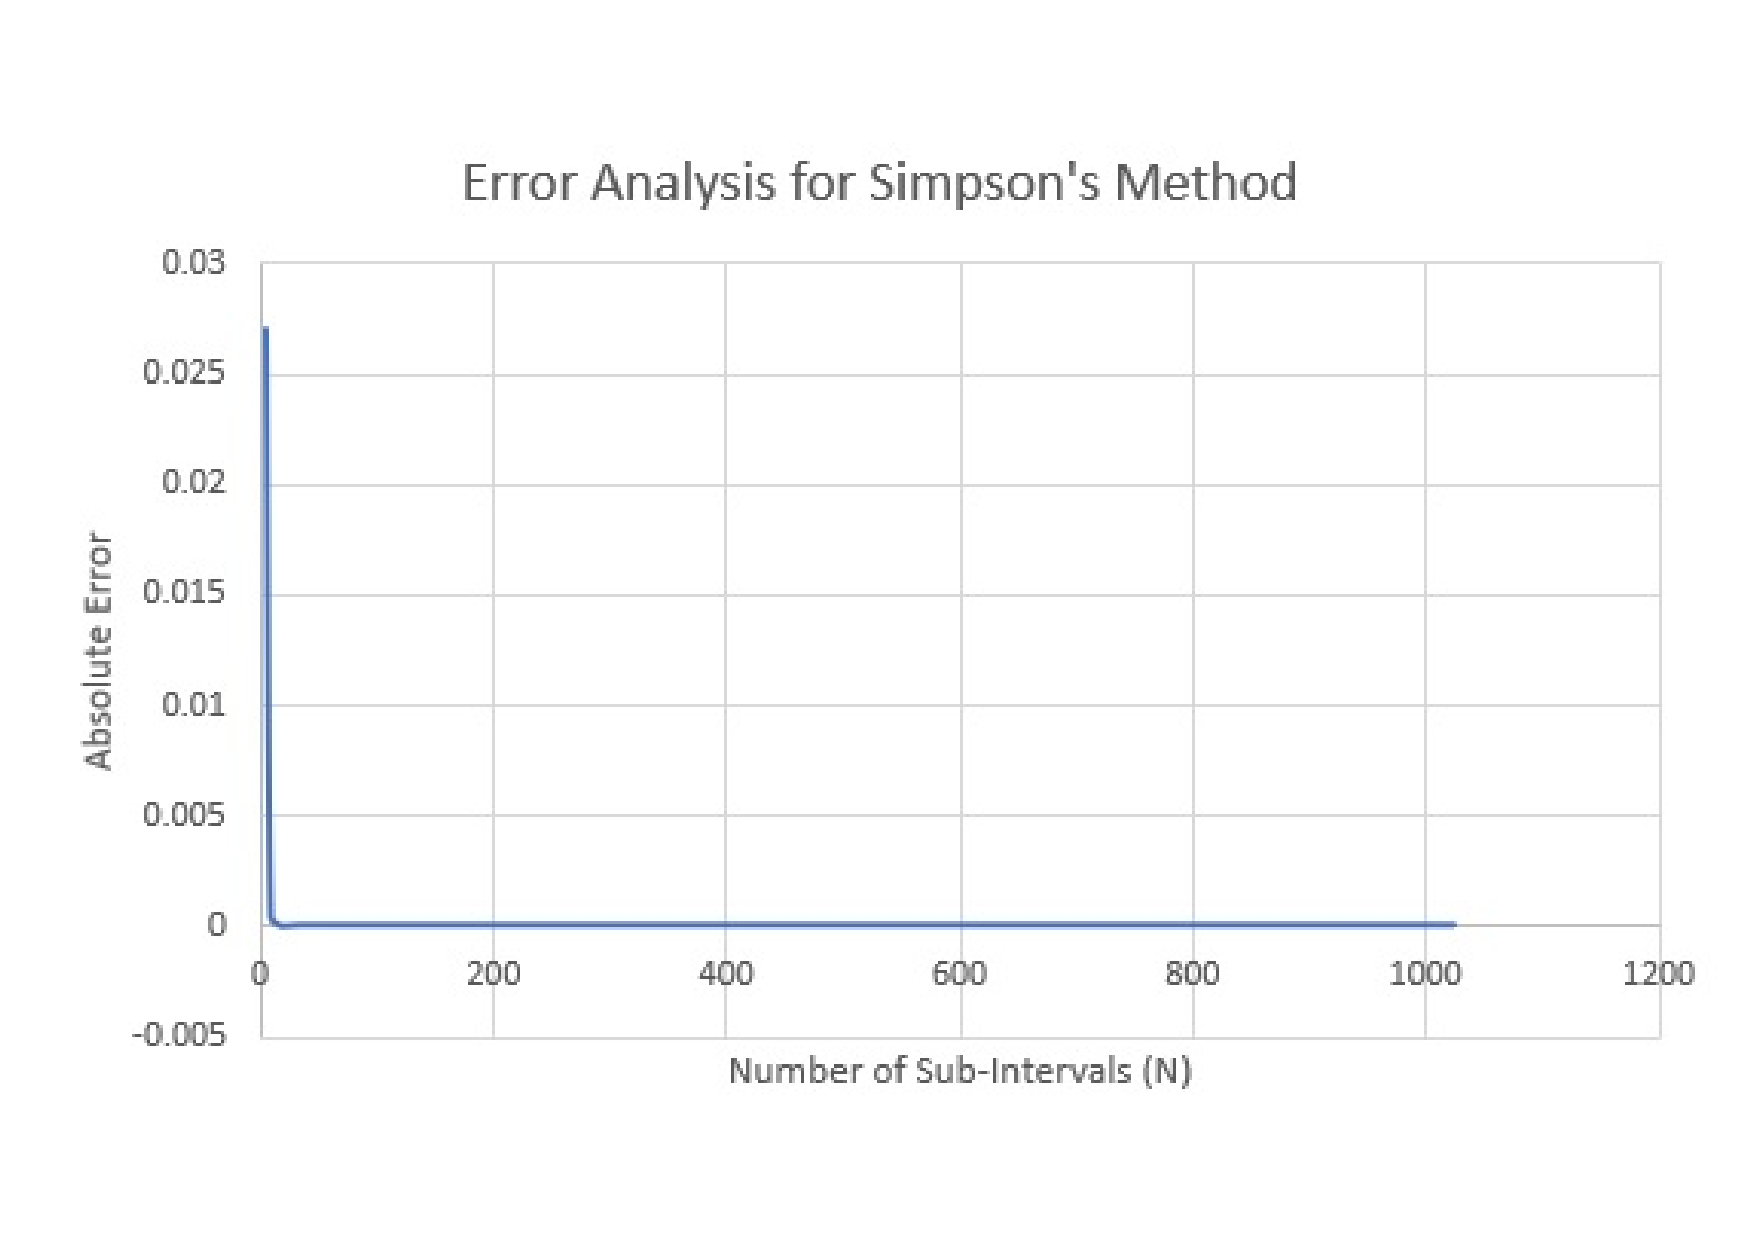
\includegraphics[width=\linewidth]{SR2ERF1.pdf}
  \caption{Error Analysis for ERF 1}
  \label{fig:q2c1}
\end{subfigure}
\begin{subfigure}{.5\textwidth}
  \centering
  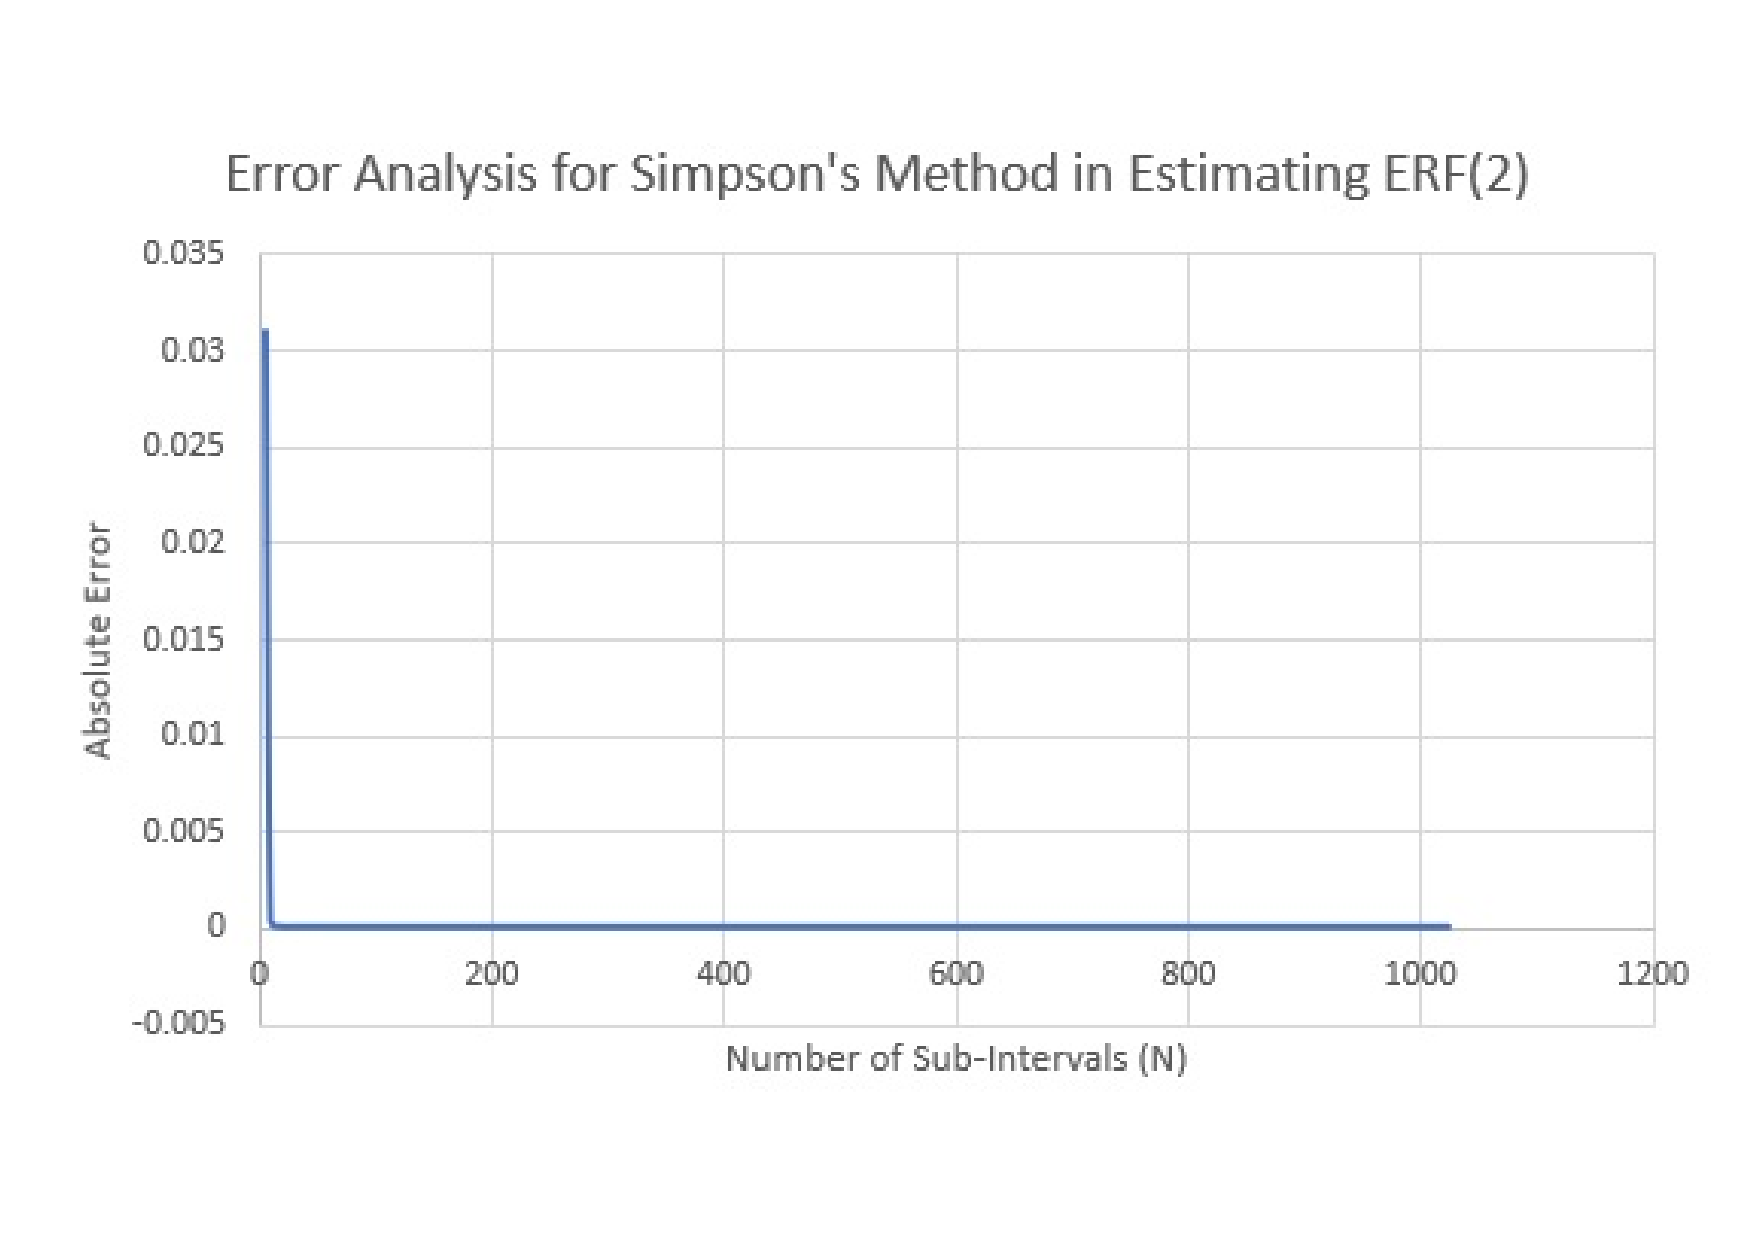
\includegraphics[width=\linewidth]{SR2ERF2.pdf}
  \caption{Error Analysis for ERF 2}
  \label{fig:q2c2}
\end{subfigure}
\caption{Absolute Error vs Number of Sub-Intervals using Simpson's $\frac{1}{3}$ Rule.}
\label{fig:q2c}
\end{figure}

Now, I tabulate my findings in two tables - one for ERF(1) and the other for ERF(2).

\begin{table}[]
    \centering
    \begin{tabular}{cccc}
        \textbf{n} & \textbf{Mid-Point} & \textbf{Trapezoid} & \textbf{Simpson's}   \\ 
       4 &	0.017415 & 0.033386	& 0.027064 \\
8&	0.004052 &	0.007985&	0.000435 \\
16 &	0.001005 & 0.001967	& 0.000008 \\
32&	0.00026 &	0.000481 &	0.000032 \\
64&	0.000075 &	0.00011 &	0.000034 \\
128&	0.000028	& 0.000018 &	0.000034 \\
256	&0.000017	&0.000005 &	0.000034 \\
512	&0.000014	&0.000011	&0.000034 \\
1024 &	0.000013&	0.000013&	0.000034 \\

    \end{tabular}
    \caption{Error Analysis for ERF(1)}
    \label{tab:Q21}
\end{table}

\begin{table}[]
    \centering
    \begin{tabular}{cccc}
        \textbf{n} & \textbf{Mid-Point} & \textbf{Trapezoid} & \textbf{Simpson's}   \\ 
    4& 0.009185&	0.01931&	0.03097 \\
8	& 0.002462	&0.005062&	0.000313\\
16	& 0.000601	& 0.0013	& 0.000046\\
32 &	0.000127 &	0.00035	& 0.000033\\
64 &	0.000008 &	0.000111 &	0.000032\\
128 &	0.000022 &	0.000052 &	0.000032\\
256	 &0.000029	& 0.000037	& 0.000032\\
512	& 0.000031	& 0.000033	& 0.000032\\
1024 & 0.000032 &	0.000032 &	0.000032\\

    \end{tabular}
    \caption{Error Analysis for ERF(2)}
    \label{tab:Q22}
\end{table}

%%%%%%%%%%%%%%%%%%%%%%%%%%%%%%%%%%%%%%%%%%%%%%%%%%%%%%

\subsection{Inferences}
I deduce the following inferences from this problem :
\begin{itemize}
    \item There is a sharp decline in the absolute error as we increase the number of sub-intervals. In principle, as n would tend towards $\intfy$, the approximate value of the integral shall converge to the true value of the integral. This is true for all the three methods demonstrated.  
    \item It appears that the \textbf{Mid Point Method} and the  \textbf{Trapezoid Method} give almost the same error. This is because both these methods approximate area using four-sided polygons - rectangle and trapezium respectively. However, \textbf{The Simpson's $\frac{1}{3}$ Rule} does much better in giving a faster convergence to the true value compared to the former methods. This is because, the Simpson's Method uses parabolas to estimate the area, which is called as \textit{The Quadratic Approximation}, and thus, does better. 
    \item Now, I shall list the various upper bounds for the error.
    \begin{itemize}
        \item [1] Error in Mid Point Method $\leq$ $\frac{M(b-a)^3}{24n^2}$
        \item [2] Error in Trapezoid Method $\leq$ $\frac{M(b-a)^3}{12n^2}$
        \item [3] Error in Simpson's Method $\leq$ $\frac{M(b-a)^5}{180n^4}$
    \end{itemize}
    where, n denotes the number of sub-intervals taken, b-a denotes the length of each sub-interval and M is the maximum modulus value of the second derivative of the function f(x).
    \item It can also be clearly inferred that the mid-point method provides a better estimate of area compared to the Trapezoid Method. The Trapezoid Method overestimates the area when the function is concave up and underestimates when the function is concave down. On the other hand, the Mid-Point method averages out the two segments. 
    \item The Simpson's Method seems to give a better and quicker approximation of the integral compared to the Mid-Point Method which in turn gives results relatively better than the Trapezoid Method.
    \item For a given n, larger the length of the interval, the upper bound on the error for the mid-point and trapezoid rule decrease while that of Simpson's Method increases. This indirectly tells us that Simpson's method is more accurate for smaller intervals as compared to larger intervals. 
    \item Similarly, for a given length of the interval, as we increase n, the upper error bound on the Mid-Point and Trapezoid rule decrease as $\frac{1}{n^2}$ while that of Simpson's rule decreases as $\frac{1}{n^4}$. This suggests that for larger number of sub-intetvals, the Simpson's rule is more accurate and quicker as compared to the other two methods.
    \item It can clearly be shown that 
    \begin{equation}
        T_n = \frac{L_n+R_n}{2}
    \end{equation}
    where $T_n$ denotes the area found using Trapezoid Rule, $L_n$ denotes the approximate integral by taking the left hand end points of each sub-interval alone and $R_n$ denotes the approximate integral by taking the right hand end points of each sub-interval alone.
    \item Simpson's Rule may be obtained from the Mid-Point and Trapezoid Rules by using a weighed average. It can be shown that :
    \begin{equation}
        S_{2n} = \frac{2M_n+T_n}{3}
    \end{equation}
    \item In summary, the Simpson's method provides a better and quicker approximate of area compared to the Mid-Point Method which in turn performs comparatively better than the Trapezoid Method.
\end{itemize}

%%%%%%%%%%%%%%%%%%%%%%%%%%%%%%%%%%%%%%%%%%%%%%%%%%%%%%

\subsection{Code}
The code used for the problem are mentioned in Listings : \begin{itemize}
    \item [1] Mid Point Rule - ~\ref{listing:4}
    \item [2] Trapezoidal Rule - ~\ref{listing:5}
    \item [3] Simpson's $\frac{1}{3}$rd Rule - ~\ref{listing:6}
\end{itemize}

\inputminted[breaklines,
 mathescape,
 linenos,
 numbersep=5pt,
 frame=single,
 numbersep=5pt,
 xleftmargin=0pt]{c}{P2MP.c}
 \captionof{listing}{Mid-Point Rule CODE}
\label{listing:4}
\inputminted[breaklines,
 mathescape,
 linenos,
 numbersep=5pt,
 frame=single,
 numbersep=5pt,
 xleftmargin=0pt]{c}{P2TP.c}
 \captionof{listing}{Trapezoidal Rule CODE}
\label{listing:5}
\inputminted[breaklines,
 mathescape,
 linenos,
 numbersep=5pt,
 frame=single,
 numbersep=5pt,
 xleftmargin=0pt]{c}{P2SR.c}
 \captionof{listing}{Simpson's $\frac{1}{3}$rd rule CODE}
\label{listing:6}

%%%%%%%%%%%%%%%%%%%%%%%%%%%%%%%%%%%%%%%%%%%%%%%%%%%%%%

\subsection{Contributions}
In the above problem, \textit{my original contributions} are - 
\begin{itemize}
    \item Designing of the Algorithm and Code
    \item Plotting of the graph on Google Sheets. 
    \item Analysis of True Error
    \item Tabulation of Results and Errors
    \item Drawing conclusions by looking at the Result obtained and Error Analysis.
    \item Writing the report in LaTeX. 
\end{itemize}


%%%%%%%%%%%%%%%%%%%%%%%%%%%%%%%%%%%%%%%%%%%%%%%%%%%%%%

\subsection{Alternate Methods}
The Mid-Point Method, Trapezoid Method and Simpson's Rule all seem to converge to the true value of the intgral as the number of sub-intervals increase. However, each of these methods has its own pitfalls. The Trapezoid method overestimates or underestimates area when subjected to concave up and concave down curvatures respectively. However, in case of linear functions, the Trapezoid and Mid-Point Methods give exact answers while Simpson's method fails to give a quicker convergence. \\
In case of unequal sub-interval lengths, the methods could perform better or worse depending on the integrand. \\
Depending on the function to be taken as the integrand. a suitable method of integration can be chosen. I shall mention few other methods here. \\
\begin{itemize}
    \item [1] \href{https://en.wikipedia.org/wiki/Romberg%27s_method}{The Romberg Method} is a more efficient method when compared to \textbf{The Simpson's $\frac{1}{3}$rd rule.}
    \item [2] \href{https://en.wikipedia.org/wiki/Boole%27s_rule}{The Boole's Rule} is also a numerical method of integration. It provides a higher efficiency compared to the three methods which we discussed in certain situations. 
    \item [3] \href{https://en.wikipedia.org/wiki/Gaussian_quadrature}{The Gaussian Quadrature} is considered in many cases as the exact integral and evaluates an integral to unexpected degree of accuracy. 
\end{itemize}
\end{document}
